\section{Matematik aflevering 1}\label{matematik-aflevering-1}

\section{9.168}\label{section}

Løs ligningen \(x^2+x-12=0\)\\
Ligningen er en andengradsligning da der er \(x^2\) og \(x\)\\
Jeg starter med at finde deskriminanten \[d = b^2-4ac\]

Værdierne for denne ligning er \(a = 1,\ b = 1,\ c = -12\)\\
Jeg indsætter dem \[d = 1^2-4 \cdot 1 \cdot -12 = 1-(-48) = 49\]

Så bruger jeg formlen \[x = \frac{-b \pm \sqrt[]{d}}{2a}\]

Jeg indsætter mine værdier

\begin{align*}
x & = \frac{-1 \pm \sqrt[]{49}}{2 \cdot 1} = \frac{-1 \pm 7}{2}\\
x & = -4 \vee x = 3
\end{align*}

Så løsningen på andengradsligningen er \(x = 4 \vee x = -0.5\)

\section{9.169}\label{section-1}

I et koordinatsystem er to vektorer \(\vec{a}\) og \(\vec{b}\) bestemt
ved
\[\vec{b} = \begin{pmatrix} 2 \\ t + 1 \end{pmatrix} \ og \ \vec{b} = \begin{pmatrix} t - 1 \\ 3 \end{pmatrix}\]

Jeg ved at hvis de skal være orthogonale skal deres prikprodukt være
\(0\) dvs.
\[\vec{a} \cdot \vec{b} = 0 \Leftrightarrow \begin{pmatrix} 2 \\ t + 1 \end{pmatrix} \cdot \begin{pmatrix} t - 1 \\ 3 \end{pmatrix} 
\Leftrightarrow 2 \cdot (t + 1) + (t - 1) \cdot 3 = 0\]

Så har vi en ligning hvor vi kan isolere og finde t
\[2t+2+3t-3=0 \Leftrightarrow 5t = 1 \Leftrightarrow t = 0.2\]

Så hvis vectorerne \(\vec{a}\) og \(\vec{b}\) skal være orthogonale skal
t være 0.2

\section{9.171}\label{section-2}

En funktion \(f\) er bestemt ved \[f(x) = e^x - x - 1\] Undersøg om
\(f\) er en løsning til differentialligningen \[\frac{dy}{dx} = y + x\]

Jeg starter med at indsætte \(f(x)\) ind på y's plads
\[\frac{dy}{dx} = e^x - x - 1 + x = e^x - 1\] Så finder jeg \(f'(x)\) og
ser om den er ens med ovenstående da \[\frac{dy}{dx} = f'(x)\]
\[f'(x)=(e^x - x - 1)'= e^x - 1\]

Jeg ser så at de er ens og derfor ved jeg at \(f(x)\) er en løsning til
differentialligningen

\section{9.175}\label{section-3}

\begin{longtable}[]{@{}rr@{}}
\toprule
Mængde & Kunder\tabularnewline
\midrule
\endhead
10 & 10\tabularnewline
20 & 23\tabularnewline
30 & 16\tabularnewline
40 & 21\tabularnewline
50 & 10\tabularnewline
60 & 9\tabularnewline
\bottomrule
\end{longtable}

Tegn en sumkurve, og bestem kvartilsættet

Jeg starter med at finde frekvensen for hvert interval ved at tage antal
kunder i intervallet og dividere det med antallet af kunder i alt

\begin{longtable}[]{@{}rrr@{}}
\toprule
Mængde & Kunder & Frekvens\tabularnewline
\midrule
\endhead
10 & 10 & 11.23596\tabularnewline
20 & 23 & 25.84270\tabularnewline
30 & 16 & 17.97753\tabularnewline
40 & 21 & 23.59551\tabularnewline
50 & 10 & 11.23596\tabularnewline
60 & 9 & 10.11236\tabularnewline
\bottomrule
\end{longtable}

Så finder jeg den kummulerede frekvens

\begin{longtable}[]{@{}rrrr@{}}
\toprule
Mængde & Kunder & Frekvens & Kumfrek\tabularnewline
\midrule
\endhead
10 & 10 & 11.23596 & 11.23596\tabularnewline
20 & 23 & 25.84270 & 37.07865\tabularnewline
30 & 16 & 17.97753 & 55.05618\tabularnewline
40 & 21 & 23.59551 & 78.65169\tabularnewline
50 & 10 & 11.23596 & 89.88764\tabularnewline
60 & 9 & 10.11236 & 100.00000\tabularnewline
\bottomrule
\end{longtable}

Så kan jeg plotte dataet ind med Mængden på x-aksen og den kummulerede
frekvens på y-aksen og aflæse hvor på grafen henholdsvis 25, 50 og 75
procent skærer grafen så jeg kan finde kvartilsættet

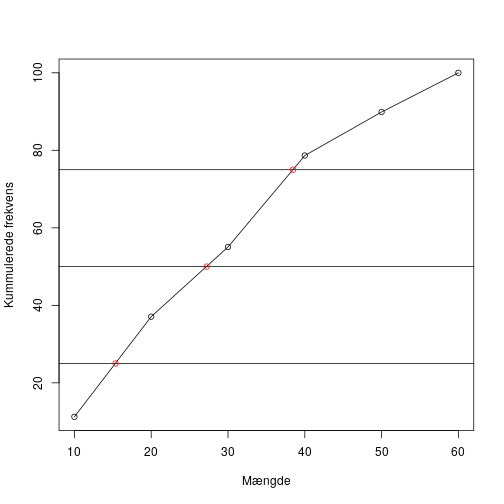
\includegraphics{figure/unnamed-chunk-4-1.png} \pagebreak

Så kan jeg så aflæse kvartilsættet på grafen til at være\\
\(Q_{1}=\) 15.4 \(median=\) 27.2 \(Q_{3}=\) 38.5

\section{9.194}\label{section-4}

SARS-epidimiens udvikling i Singapore i 2003 kan beskrives ved
differentialligningen \[\frac{dN}{dt}=0.00526 \cdot N \cdot (209 - N)\]
hvor \(N\) er antal smittede til tidspunktet \(t\) (målt i døgn). Det
oplyses, at der efter 30 døgn car 103 smittede.

\begin{enumerate}
\def\labelenumi{\arabic{enumi}.}
\item
  Jeg indsætter bare 100 ind i differentialligningen da det er det
  eneste variable på højre side af ligningen.
  \[\frac{dN}{dt}=0.00526 \cdot 100 \cdot (209 - 100) = 57.334\] Så
  væksthastigheden da antal smittet var 100 ville være 57.334 smittede
  pr døgn
\item
  Jeg kan se på differentialligningen at det er logistisk vækst som
  følger modellen \[\frac{dy}{dx}=ay \dot (M - y)\] Så jeg kan bare
  indsætte værdierne ind i skabelonen

  \begin{align*}
  y & = f(x) = \frac{M}{1+ce^{-aMx}}\\
  N(t) & = \frac{209}{1+ce^{-0.00526 \cdot 209 \cdot t}} = \frac{209}{1+ce^{1.09934t}}
  \end{align*}

  Tallet 209 i differentialligningen betyder at \(N(t)\) aldrig vil gå
  over 209 det ville kun kunne komme meget tæt på
\end{enumerate}

\section{9.200}\label{section-5}

Bestem integralet \[\int \frac{2x}{x^2+3} \ dx\] Jeg starter med at
skubbe tælleren ned da jeg vil bruge substitutionsmetoden
\[\int \frac{1}{x^2+3} \cdot 2x \ dx\] Jeg sætter \(t\) til at være
\(x^2+3\)

\begin{align*}
t & = x^2+3\\
t' & = 2x\\
\frac{dt}{dx} & = 2x \Leftrightarrow dt = 2x \ dx
\end{align*}

Så substituerer jeg det ind i integralet \[\int \frac{1}{t} \ dt\] Nu er
den lidt mere overskuelig, og da jeg ved at
\(\int \frac{1}{x} = ln(x)+k\) ved jeg at integralet så er
\[\int \frac{1}{t} \ dt = ln(t)+k\] Så substituere jeg tilbage
\[ln(t) = ln(x^2+3)+k\] Så stamfunktionen til \(\frac{2x}{x^2+3}\) er
\(ln(x^2+3)+k\)
